\subsubsection{UC9 - Gestione prenotazione}
 \begin{figure}[h]
	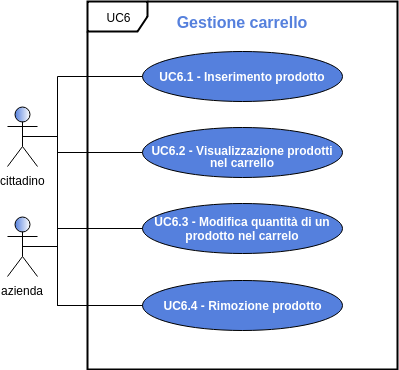
\includegraphics[width=6cm]{res/images/UC6GestioneCarrello.png}
	\centering
	\caption{UC6 - Gestione prenotazione}
\end{figure}
\begin{itemize}
	\item \textbf{Attori Primari}: utente autenticato;
	\item \textbf{Descrizione}: agli utenti autenticati è resa disponibile una maschera che presenta la lista di tutte le sue prenotazioni, dalla quale l'utente può scegliere di effettuare operazioni di gestione su ognuna di esse;
	Per ogni prenotazione presente nella lista saranno visualizzati dei dettagli riassuntivi, che sono:
	\begin{itemize}
		\item \textit{da completare in seguito}.
	\end{itemize}
	\item \textbf{Scenario principale}: l'utente effettua operazioni di gestione di una prenotazione. Esse comprendono:
	\begin{enumerate}[label=\alph*.]
		\item la visualizzazione dei dettagli di una prenotazione [UC6.1];
		\item la modifica di una prenotazione [UC6.2];
		\item la cancellazione di una prenotazione [UC6.3].
	\end{enumerate}
	\item \textbf{Precondizione}: il sistema riconosce l'utente proprietario o usufruente e rende disponibile il servizio di gestione delle prenotazioni;
	\item \textbf{Post-condizione}: l'utente riconosciuto può procedere con le operazioni di gestione rese disponibili.
\end{itemize} 
 \subsubsection{UC6.1 - Visualizzazione dettagli prenotazione}
\begin{itemize}
	\item \textbf{Attori Primari}: utente autenticato;
	\item \textbf{Descrizione}: l'utente visualizza i dettagli della prenotazione scelta dalla maschera di presentazione delle prenotazioni;
	\item \textbf{Scenario principale}:
	\begin{enumerate}[label=\alph*.]
		\item l'utente sta visualizzando i dettagli della prenotazione;
		\item l'utente sceglie di modificare la prenotazione scelta [UC6.2];
		\item l'utente sceglie di eliminare la prenotazione scelta [UC6.3].
	\end{enumerate}
	\item \textbf{Precondizione}: l'utente sta visualizzando i dettagli della prenotazione scelta dalla maschera di presentazione delle prenotazioni;
	\item \textbf{Post-condizione}: l'utente ha visualizzato e/o modificato la prenotazione precedentemente scelta.
\end{itemize}

\subsubsection{UC6.2 - Modifica di una prenotazione}
\begin{itemize}
	\item \textbf{Attori Primari}: utente autenticato;
	\item \textbf{Descrizione}: l'utente modifica uno o più dati della prenotazione selezionata;
	\item \textbf{Scenario principale}: l'utente si trova all'interno della pagina di modifica della prenotazione precedentemente selezionata;
	\item \textbf{Precondizione}: l'utente si trova nella pagina di presentazione di tutte le sue prenotazioni e ne ha selezionato una per la modifica, oppure l'utente si trova nella pagina di visualizzazione dettagli prenotazione e sceglie di modificare quest'ultima;
	\item \textbf{Post-condizione}: l'utente ha modificato uno o più dati della prenotazione selezionata.
\end{itemize}

\subsubsection{UC6.3 - Cancellazione di una prenotazione}
\begin{itemize}
	\item \textbf{Attori Primari}: utente autenticato;
	\item \textbf{Descrizione}: l'utente cancella la prenotazione selezionata;
	\item \textbf{Scenario principale}: l'utente si trova all'interno della pagina di cancellazione della prenotazione precedentemente selezionata. Verrà chiesta conferma all'utente prima di procedere con la cancellazione;
	\item \textbf{Precondizione}: l'utente si trova nella pagina di presentazione di tutte le sue prenotazioni e ne ha selezionato una per la cancellazione, oppure l'utente si trova nella pagina di visualizzazione dettagli prenotazione e sceglie di cancellare quest'ultima;
	\item \textbf{Post-condizione}: l'utente ha confermato o annullato la cancellazione della prenotazione selezionata.
\end{itemize}
